\documentclass{mpaper}

\usepackage{graphicx}
\usepackage[numbers,sort&compress]{natbib}
\usepackage{algorithm}
\usepackage{algpseudocode}
\usepackage{amsmath}
\usepackage[table,xcdraw]{xcolor}

\begin{document}

\title{Statistical Model Updates in Distributed Computing:\\ An Optimal Stopping Theory Perspective}
\author{Ekaterina Aleksandrova}
\matricnum{2133352a}

\maketitle

\begin{abstract}
This paper explores a sequential decision making methodology of \textit{when to update} statistical learning models in Intelligent Edge Computing Devices given underlying changes in the contextual data distribution. The proposed model update scheduling takes into consideration the optimal decision time for minimizing the network overhead while preserving the prediction accuracy of the models. The paper reports on a comparison between the proposed approach with four other update delaying policies found in the literature, an evaluation of the performances using linear and support vector regression models over real contextual data streams and a discussion on the strengths and weaknesses of the proposed policy.
\end{abstract}

\section{Introduction}
The Internet of Things (IoT) environments have been gaining popularity since the end of the 20th century. They have allowed the transformation of small computing environments into large scale ecosystems, whose cores (cloud data centers) require a massive computational 
power to process all the received contextual data along with a substantial network overhead in order to receive all the raw data.

However, as this has proven to be inefficient, a computing paradigm has been provided in the form of Edge Computing (EC), whose rationale is to \textit{push most of the computations to the edge of the network}, e.g. sensors, mobile devices, etc. This allows to take advantage of the computational and sensing capabilities of modern devices and deliver the locally processed contextual data to the cloud in the form of partially or entirely extracted knowledge \cite{anagnostop2014}.
The edge-centric rationale also contributes as a security measure as raw data is processed locally on the sensing device and as a method for decreasing network traffic, as the delivered statistical learning model representations of the data have significantly smaller size compared to the raw contextual sensed data. The EC methodology is expected to significantly reduce the required computational power. However, if the acquired knowledge is still transferred to the Cloud on each iteration, then the considerable communication overhead remains along with other complications explained further ahead in this paper. 

\subsection*{Problem Statement}
The main problem which this work aims is to estimate an \textit{optimal waiting time criteria} based on made sequential observations on multivariate contextual data. The proposed scheme should be able to decide when a model representation of the sensed data is to be sent from an edge node to an edge gateway in order to minimise the communication overhead and, in parallel, to preserve or increase the accuracy of the generated statistical models. This can be expressed as the following research question:

\textbf{How can the delivery waiting time and model accuracy at the edge gateway be maximised while minimising the communication overhead and computational complexity at the sensing edge node level?}

\subsection*{Paper Organisation}
The paper is organised as follows: Section 2 presents related work on the current state of the art on this research topic. Section 3 introduces the proposed methodology followed for this project including the rationale behind the proposed algorithm built on the principles of the Optimal Stopping Theory. Section 4 reports on the performance assessment and comparison of the proposed method with other sequential decision making policies and algorithms using real data sets and provides a summarised analysis. Section 5 includes the concluding remarks and ideas on future development of this work.

\section{Related Work \& Background}
\subsection{Knowledge Sharing in IoT Environments}
Given a sample path in an IoT system consisting of multiple sensing nodes, 
a local edge gateway and a central data node as en endpoint, 
the multi-hop transmission can increase energy consumption when the gateway is busy and the data has to be passed to the central node \cite{shi2016}. 
When data processing is not performed at the edge level, 
if $N$ multivariate data points are sensed and sent through the network, 
that results in $N$ number of transmissions. However, 
if the data $X$ is locally processed at the edge, the result 
can be a linear model representation of the data e.g., $y = \alpha \cdot X + \beta$, 
where only the parameters $\alpha, \beta$ are being passed through the network resulting in a reduced energy consumption \cite{tanluizhang2011}.

Wireless Sensor Networks (WSNs) in IoT environments used in remote locations (e.g. rain forest sensors  \cite{rainforests2009}, surface and mine monitoring \cite{Akkas2018}, water pollution detectors\cite{waterwsn2017}, etc.) are usually being powered by a battery. 
Therefore, the energy consumption of the sensing devices should be minimised as much as possible to reduce the amount of human interaction required to replace the exhausted energy source. 
Such interaction with the device may distort the environment and introduce incorrect data. 
If the sensors are placed at locations with difficult access, that could also increase the financial cost or even cause danger to the person responsible for the replacement.

Other similar sensor systems rely on renewable energy, most widely used is solar energy, which could be slower to harvest in environments such as rain forests \cite{rainforests2009}, 
therefore, having a power efficient device is required in order to have a well-functioning system. Another concern with communicating processed data on every sensing \& reporting iteration is that it is possible that the data contains bias, e.g. missing or corrupted data points \cite{anagnostop2016}. When passed to the gateway it can potentially be used to make inaccurate predictions of the sensed environment. This can be avoided by \textit{delaying} the model update before making sure that the bias is not in fact a novelty in the data.

A way of minimising the energy cost of an edge device even more is by reducing the number of the data transmissions. This could be performed by introducing a certain delay in the delivery of the up-to-date model \citep{anagnostop2014, anagnostop2016, anagnostopkolomvatos2016}, at the cost of allowing a reasonable error in the data. Based on this delay-based rationale, the approach adopted in this work is as follows: \textit{a data model is generated at the edge node and then sent to the edge gateway, on the next iteration. In the case that the node does not detect a significant change between the initially modelled data and the currently sensed dataset, 
no communication is made between the edge node and the edge gateway. 
Making the decision when to send a new updated model to the edge gateway before the accuracy has degraded beyond a reasonable threshold should be looked from a slightly different angle.} 

\subsection{Time-optimised Decision Making on Changes}
The Optimal Stopping Theory (OST) attempts to solve exactly the problem stated above, i.e., choosing a \textit{best} time instance to take a given action: 
stop observing changes on the derived model and send the model to the edge gateway. 
The action is based on sequentially observed random variables from a distribution in order to maximise an expected reward or minimise an expected cost. Based on this abstraction of the considered problem, several OST-based variations are adopted as a basis to problems in Computing Science notably: the called \emph{House-Selling} problem and the \emph{Quickest Change Detection} problem \cite{UCLAbook}.  

The House-Selling problem explores the attempt to stop and sell a house at the highest offer by taking into account a cost, such as living cost or real estate agency commission, for each rejected offer. 
This problem relates to the approach that waiting can be penalised, the way Tian et al. use it in their "cost-aware" update policy algorithm \cite{tian18}. In our context, the decision on whether to update an outdated statistical learning model with the current one is based on how much it was lost (how big the "regret" is) since the update with the better model was not performed in the past. 
Once a tolerance threshold is passed, an update is inevitable, which also prevents additional retraining computations on the edge node. 

The Change Point Detection problem deals with the exploration of the context distribution and stopping when a change is detected but penalising when the algorithm has signalled a false alarm \cite{UCLAbook}. Research has been mainly focusing on two major approaches based on assumptions on the underlying data distribution. 
Shiryaev \cite{shiryaev1963} provides an optimal solution to the problem using a Bayesian approach. While, on the other hand, there is a non-Bayesian approach using the well-known CuSum algorithm provided by Page \cite{page1954}. The latter was proven to be optimal by Moustakides \cite{moustakides1986} based on Lorden's formulation of the problem \cite{lorden1971}.

In a recent publication, Lau and Tay\cite{lautay2018} introduce the idea of having a "critical change" and a "nuisance change" in a distribution, where the critical change is of highest importance and should be detected, as opposed to the nuisance change which should be ignored by the algorithm. They propose two algorithms using a Bayesian and a non-Bayesian approach, which then are compared to the performance for both types of change against the naive 2-stage procedures by Page\cite{page1954} and Shiryaev\cite{shiryaev1963}.
For their non-Bayesian approach, the authors compare their proposed algorithm with the naive 2-stage CuSum. The naive approach uses two separate thresholds, $\beta_c$ for the critical change and $\beta_n$ for the nuisance change. First they are applied on the cumulative sum of the log-likelihood ratio of the normal distribution and then on the distributions after the nuisance and the critical change. According to the authors, their non-Bayesian procedure, which is based on the Generalised Likelihood Ratio test, performs more accurately than the naive 2-stage optimal CuSum algorithm.

\subsection{Contribution}
The contributions of this paper are as follows:
\begin{enumerate}
\item An analytical optimisation model derived from the optimal stopping rule aimed at minimising the communication overhead at EC systems.
\item A comparison of the derived rule to an established change detection rule and an intuitive base method
\item A method for hyperparameter optimisation when applying the optimal postponing rule
\end{enumerate}

\section{Methodology}
The main focus of this work is to present and experiment with the
proposed \textit{time-optimised model update postponing} policy/algorithm for reducing the communication rate but preserving the quality of the context. We assume that the distributed/EC environment contains at least sensor node and an edge gateway device. 

Initially, the sensing node is responsible for gathering environmental / multivariate contextual data and generating a statistical/Machine Learning (ML) model from the first \textbf{\emph{w}} contextual data observations. The ML model is then temporarily stored on the sensing device but also is communicated with the edge gateway. 
On each next observation, the piece of data is received and appended to the currently stored sensor data set of size \textbf{\emph{w}}, while the datum with the oldest timestamp is discarded. 
A new model is generated or incrementally updated representing the current updated dataset. By fitting the dataset on the old and the new ML models, we obtain the two Mean Squared Errors (MSE):
\begin{itemize}
    \item MSE \textbf{$e$} from the ML model the edge gateway, which has been previously received;
\item MSE \textbf{$e'$} from the ML model based on the most up-to-date sensed data at the edge node.
\end{itemize}

Given that the predictability of the latest ML model of the edge node satisfies a certain criteria, the decision is made to communicate the current ML model to the edge gateway. This also requires that the temporarily stored outdated ML model at the edge device is also updated to correctly represent the disseminated local knowledge in the eco-system.

\subsection{Optimal Postponing Policy}
The Optimal Postponing (OP) policy for ML model update is based on the change in the distribution using the cumulative sum of the absolute error difference between the two MSEs $e$ and $e'$ at time instance/observation $t>0$. Consider the following definitions:
\begin{align}
    Z_t &= \Delta e_t = | e'_t - e_t |\\
    S_{t+1} &= \Delta e_{t+1} + \Sigma_{k=0}^t \Delta e_k\\
    S_t &= S_{t-1} + Z_t\label{eq:1}
\end{align}

An error tolerance threshold $\Theta > 0$ is defined to determine the acceptable error sum, which will be used to determine if the 
edge node should proceed with a ML model update to the edge gateway or not. Under this context, we define the following random variable $V_{t}$ as the reward of an update decision:
\begin{equation}\label{reward}
    V_t = \Bigg\{ \begin{tabular}{c}
                  $t,\ \text{if}\ S_t \leq \Theta$, \\
                  $-B,\ \text{if}\ S_t > \Theta.$
                  \end{tabular}
\end{equation}

The penalty factor $B> 0$ denotes that the current cumulative error exceed the error tolerance $\Theta$, thus, the edge node could have sent the updated ML model to the edge gateway. On the other hand, to be communication efficient, the edge node desires to postpone the ML model update, thus, increasing the value of $V_{t}$. However, as long as the edge node delays the model update, then the cumulative error $S_{t}$ approaches $\Theta$. The problem is for the cumulative error $S_{t}$ to reach as close to the tolerance $\Theta$ as possible, but without exceeding this. Hence, we then formalise the OST problem:

\textbf{Problem 1} The edge node should find the best time instance $t^{*}$ such that the expected reward for delaying a ML model update is maximized, i.e., the optimal stopping time $t^{*}$ obtains the following essential supremum
\[
\mbox{ess} \sup_{t} \mathbb{E}[V_{t}].
\]

We then provide the solution of the optimal stopping time estimate as stated in the Theorem 1.
\\
\\
\textbf{Theorem 1}\textit{
The optimal stopping time $t^{*}$ that maximizes the essential supremum $\mbox{ess} \sup_{t} \mathbb{E}[V_{t}]$ of the reward function on the edge node is the first time instance $t>0$ such that:
\[
F_{Z}(\Theta - S_{t}) \leq \frac{t+B}{t+1+B},
\]
where $F_{Z}(z)$ is the cumulative distribution function (CDF) of the error differences $Z_{t}$ of the old and the updated ML models $e_{t}$ and $e_{t}'$, respectively.}  
\\

% Taking into consideration that the expected reward $E[V_t]$ must be a positive value, we can calculate the probability interval that the cumulative sum is less than or equal to the set threshold.
% \begin{equation}
%     P(S_t \leq \Theta) > \frac{B}{t+B}
% \end{equation}
% \emph{\textbf{Proof:}} \\

\textbf{Proof of Theorem 1}
From the reward function in (\ref{reward}) we can derive the expected current reward $\mathbb{E}[V_t]$. 
\begin{equation}
\begin{split}
    \mathbb{E}[V_t] & = t \cdot P(S_t \leq \Theta) + (-B \cdot P(S_t > \Theta))\\
    & = t \cdot P(S_t \leq \Theta) - B \cdot (1 - P(S_t \leq \Theta))\\
    & = (t + B) \cdot P(S_t \leq \Theta) - B,
\end{split}
\end{equation}
Let now the filtration $\mathbb{F}_{t} = \{S_{1}, S_{2}, \ldots, S_{t}\} \cup \{Z_{1}, Z_{2}, \ldots, Z_{t}\}$ be the realisation of all random variables up to $t$. This is the whole information the edge node has accumulated up to time instance $t$. 
Then, the conditional expectation of the reward $V_{t+1}$ given filtration $\mathbb{F}_{t}$ is then expressed as a martingale:

\begin{eqnarray}
    \mathbb{E}[V_{t+1}|\mathbb{F}_{t}] & = & (t + 1 + B) \cdot P(S_{t+1} \leq \Theta | \mathbb{F}_t) - B
\end{eqnarray}

However, it is known from Eq.(\ref{eq:1}) that:
\begin{equation}
    S_{t+1} = S_t + Z_{t+1}
\end{equation}
Therefore, the probability of the sum at time instance $t+1$ being less then or equal to $\Theta$ given filtration $\mathbb{F}$ equals the cumulative distribution function of $Z$ taking a value less than or equal to $\Theta - S_t$ 
\begin{align*}
    P(S_{t+1} \leq \Theta | \mathbb{F}_t) &= P(S_t + Z_{t+1} \leq \Theta| \mathbb{F}_t)\\
                           &= P(Z_{t+1}\leq\Theta-S_t| \mathbb{F}_t)\\
                           &= F_{Z}(\Theta - S_t)
\end{align*}
Hence, we obtain that:
\begin{align*}
    \mathbb{E}[V_{t+1}|\mathbb{F}_{t}] &= (t + 1 + B) \cdot P(S_{t+1} \leq \Theta | \mathbb{F}_t) - B\\
    &=(t + 1 + B) \cdot P(S_{t}+Z_{t+1} \leq \Theta | \mathbb{F}_{t}) - B\\
    &=(t + 1 + B) \cdot P(Z_{t+1} \leq \Theta-S_{t+1} | \mathbb{F}_{t}) - B\\
    &=(t + 1 + B) \cdot F_{Z}(\Theta-S_{t}) - B\\
\end{align*}

We aim to postpone sending the ML model if we know that the next iteration will increase the reward value. That is why we stop at the first instance $t$ where the current reward is more than the expected future reward at time instance $t+1$ or $V_{t} \geq \mathbb{E}[V_{t+1}|\mathbb{F}_{t}]$. Based on this, we obtain that:

\begin{eqnarray}
    V_t & \geq  & \mathbb{E}[V_{t+1}|\mathbb{F}_t] \\
    t & \geq  & (t+1+B)\cdot F_{Z}(\Theta - S_t) - B\\
    F_{Z}(\Theta - S_t) &\leq & \frac{t+B}{t+1+B},
\end{eqnarray}
which completes the proof of Theorem 1. 
\qed

Algorithm \ref{polOP} illustrates the local process in the edge node. 

% \begin{algorithm}
% \caption{Time-optimised Policy (OP)}\label{polOP}
% \begin{algorithmic}
% \State $rewardDist \gets$ obtainRewardDist() \Comment{Apendix \ref{rewarddist}}
% \State $X_0, y_0\gets$ fromDataStream
% \State $X_1, y_1 \gets$ fromDataStream
% \State $initModel \gets$ fit($X_0, y_0$)
% \State $model \gets$ fit($X_1, y_1$)
% \State $mse \gets$ calcError($initModel,X_1,y_1$)
% \State $msePrime \gets$ calcError($model,X_1,y_1$)
% \State $absError \gets \mid mse - msePrime \mid$
% \State $absErrorSum \gets absError$
% \While{$True$}
%     \State $X, y \gets$ fromDataStream
%     \State $newModel \gets$ fit($X,y$)
%     \State $mse \gets$ calcError($model,X,y$)
%     \State $msePrime \gets$ calcError($newModel,X,y$)
%     \State $absError \gets \mid mse - msePrime \mid$
%     \If{cdf($rewardDist, (\Theta-absErrorSum$)) $\leq$\\\hspace{4.4cm} $(t+B)/(t+1+B)$}
%         \State $model \gets newModel$ \Comment{communicate model}
%         \State $absErrorSum \gets absError$
%         \State $t \gets 0$
%     \Else
%         \State $absErrorSum \gets absErrorSum + absError$
%     \EndIf
%     \State $t \gets t + 1$
% \EndWhile
% \end{algorithmic}
% \end{algorithm}

\begin{algorithm}
\caption{Time-optimised Policy (OP)}\label{polOP}
\begin{algorithmic}
\State $rewardDist \gets$ obtainRewardDist() \Comment{Appendix \ref{rewarddist}}
\State \textbf{receive}($X_0, y_0, X_1, y_1$)
\State $initModel \gets$ \textbf{fit}($X_0, y_0$)
\State $model \gets$ \textbf{fit}($X_1, y_1$)
\State $e \gets$ \textbf{error}($initModel,X_1,y_1$)
\State $e' \gets$ \textbf{error}($model,X_1,y_1$)
\State $Z \gets \mid e - e' \mid$
\State $S \gets Z$; $t \gets 1$
\While{$true$}
    \State \textbf{receive}($X, y$)
    \State $newModel \gets$ \textbf{fit}($X,y$)
    \State $e \gets$ \textbf{error}($model,X,y$)
    \State $e' \gets$ \textbf{error}($newModel,X,y$)
    \State $Z \gets \mid e - e' \mid$
    \If{\textbf{cdf}($rewardDist, (\Theta-S$)) $\leq \frac{t+B}{t+1+B}$}
        \State $model \gets newModel$ \Comment{update \& communicate model}
        \State $S \gets Z$; $t \gets 1$
    \Else
        \State $S \gets S + Z$; $t \gets t + 1$
    \EndIf
\EndWhile
\end{algorithmic}
\end{algorithm}
\newpage
\subsection{Policies under Comparison}
In order to evaluate the performance of the presented algorithm 4 other policies are implemented, which rely either on certain statistics of the data or on pure randomness: the Median-based Policy, the Random Policy, the Accuracy Policy, and the optimal CuSum Policy \cite{cusum_pierre}.

\subsubsection{Median-based Policy}
The Median Policy has an initially learned median from the previously seen data. It is calculated from the absolute error difference values given that the initial model is never updated. 
The rationale behind this is to explore the worst case scenario of the error difference. This assumes that the closer the timestamps of two models are, the lower the error difference between them is and on the contrary, the further away the timestamps of two models are, the higher their error difference is.

Using a fraction $\alpha$ of the median value the policy determines whether the current absolute error difference is a tolerable amount or if it indicates that the newly sensed data is significantly outdated and needs to be communicated with the edge gateway.

This policy is expected to reduce communication by being more tolerant towards initial small abrupt changes but detects continuously increasing values.

% \begin{algorithm}[h!]
% \caption{Median-based Policy}\label{polM}
% \begin{algorithmic}
% \Procedure{obtainMedian}{}
%     \State $X, y \gets$ fromDataStream
%     \State $model \gets$ fit($X,y$)
    
%     \For{$i = 0$ \textbf{to} $100$}
%         \State $X, y \gets$ fromDataStream
%         \State $newModel \gets$ fit($X,y$)
%         \State $mse \gets$ calcError($model,X,y$)
%         \State $msePrime \gets$ calcError($newModel,X,y$)
%         \State $all \gets \mid error - msePrime \mid$
%     \EndFor
%     \State $median \gets$ calcMedian($all$)
% \EndProcedure

% \State $X, y \gets$ fromDataStream
% \State $model \gets$ fit($X,y$)
% \While{$True$}
%     \State $X, y \gets$ fromDataStream
%     \State $newModel \gets$ fit($X,y$)
%     \If{$\mid error - msePrime \mid > \alpha \cdot median$}
%         \State $model \gets newModel$ \Comment{communicate model}
%     \EndIf
%     \If{$iteration \mod 100 = 0$}
%         \State updateMedian()
%     \EndIf
% \EndWhile
% \end{algorithmic}
% \end{algorithm}

\begin{algorithm}[h!]
\caption{Median-based Policy}\label{polM}
\begin{algorithmic}
\Procedure{obtainMedian}{}
    \State \textbf{receive}($X, y$)
    \State $model \gets$ \textbf{fit}($X,y$)
    
    \For{$t \gets 1$ \textbf{to} $T$}
        \State \textbf{receive}($X, y$)
        \State $newModel \gets$ \textbf{fit}($X,y$)
        \State $e \gets$ \textbf{error}($model,X,y$)
        \State $e' \gets$ \textbf{error}($newModel,X,y$)
        \State $E \gets E \cup \{\mid e - e' \mid\}$
    \EndFor
    \State $median \gets$ \textbf{median}($E$)
\EndProcedure
\State \textbf{receive}($X, y$)
\State $model \gets$ \textbf{fit}($X,y$)
\While{$true$}
    \State \textbf{receive}($X, y$)
    \State $newModel \gets$ \textbf{fit}($X,y$)
    \State $e \gets$ \textbf{error}($model,X,y$)
    \State $e' \gets$ \textbf{error}($newModel,X,y$)
    \If{$\mid e - e' \mid > \alpha \cdot median$}
        \State $model \gets newModel$ \Comment{update \& communicate model}
    \EndIf
    \If{$t \mod T = 0$}
        \State \textbf{updateMedian}()
    \EndIf
\EndWhile
\end{algorithmic}
\end{algorithm}

\subsubsection{Random-based Policy}
The random policy is intended to be sending updates of the latest model to the edge gateway with the same probability as the OST policy.

The aim of the policy is to show that even if the number of updates is approximated to the optimal value, the accuracy of the models at the edge gateway would still suffer a decrease.

\begin{algorithm}[h]
\caption{Random-based Policy}\label{polR}
\begin{algorithmic}
\State  \textbf{receive}($X,y$)
\State $model \gets$ \textbf{fit}($X,y$)

\While{$true$}
    \State \textbf{receive}($X, y$)
    \State $newModel \gets$ \textbf{fit}($X,y$)
    \State $rand \gets$ \textbf{generate}($\{0,1\},probability$)
    \If{$rand = 1$}
        \State $model \gets newModel$ \Comment{update \& communicate model}
    \EndIf
\EndWhile
\end{algorithmic}
\end{algorithm}

% \begin{algorithm}[h]
% \caption{Random-based Policy}\label{polR}
% \begin{algorithmic}
% \State $X,y \gets$ fromDataStream
% \State $model \gets$ fit($X,y$)

% \While{$True$}
%     \State $X, y \gets$ fromDataStream
%     \State $newModel \gets$ fit($X,y$)
%     \State $rand \gets$ genZeroOrOne($probability$)
%     \If{$rand = 1$}
%         \State $model \gets newModel$ \Comment{communicate model}
%     \EndIf
% \EndWhile
% \end{algorithmic}
% \end{algorithm}

\subsubsection{Accuracy-based Policy}
The accuracy policy works by comparing the MSE of the old model and the most up-to-date model. Once it detects a decrease in the accuracy the latest model is sent to the edge gateway.
The policy aims to present a naive algorithm for reducing communication but preserving accuracy as high as possible.

% \begin{algorithm}[h]
% \caption{Accuracy-based Policy}\label{polA}
% \begin{algorithmic}
% \State $X, y \gets$ fromDataStream
% \State $model \gets$ fit($X,y$)

% \While{$True$}
%     \State $X, y \gets$ fromDataStream
%     \State $newModel \gets$ fit($X,y$)
%     \State $mse \gets$ calcError($model, X, y$)
%     \State $msePrime \gets$ calcError($newModel, X, y$)
%     \If{$mse > msePrime $}
%         \State $model \gets newModel$ \Comment{communicate model}
%     \EndIf
% \EndWhile
% \end{algorithmic}
% \end{algorithm}

\begin{algorithm}[h]
\caption{Accuracy-based Policy}\label{polA}
\begin{algorithmic}
\State  \textbf{receive}($X, y$)
\State $model \gets$ \textbf{fit}($X,y$)
\While{$true$}
    \State \textbf{receive}($X, y$)
    \State $newModel \gets$ \textbf{fit}($X,y$)
    \State $e \gets$ \textbf{error}($model, X, y$)
    \State $e' \gets$ \textbf{error}($newModel, X, y$)
    \If{$e > e' $}
        \State $model \gets newModel$ \Comment{update \& communicate model}
    \EndIf
\EndWhile
\end{algorithmic}
\end{algorithm}

\subsubsection{CuSum Policy}
The algorithm implemented here relies on the direct form of the CuSum algorithm explained by Granjon \cite{cusum_pierre}.

For the execution of the algorithm, two assumptions of the distributions are made representing the two hypothesis, where the algorithm aims to decide which hypothesis represents the current sample of data. 
Firstly, the $\mathcal{H}_0$ no change hypothesis refers to the "good distribution" which is assumed to be the distribution of the absolute error difference when the edge gateway model is communicated on every iteration. On the contrary, the "bad distribution" represented by the changed distribution hypothesis $\mathcal{H}_1$ is assumed to be the distribution of the absolute error difference when the model is communicated only on the first iteration and then never again.

The assumption is made that the absolute error differences $Z_0, Z_1, \dotsc , Z_n $ are continuous independent random variables. In this case a gamma distribution is a good choice to represent the data  [Fig.\ref{fig:goodvsbad}], relying on the two flexible parameters for scale and shape of the probability density function of the distribution.

\begin{figure}[h]
    \centering
    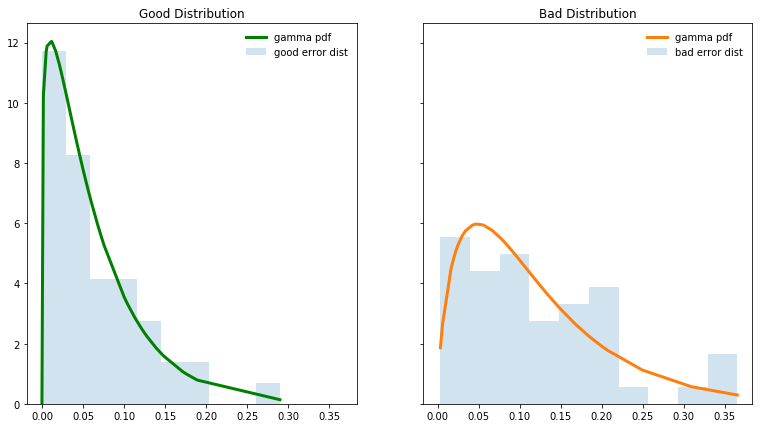
\includegraphics[scale=0.3]{imgs/goodVSbad.png}
    \caption{Gamma distribution approximation on GNFUV data using Linear Regression}
    \label{fig:goodvsbad}
\end{figure}

When a new absolute error difference is calculated it is then fitted in the probability density function for each of the two distributions. The logarithmic ratio of the probability of the absolute error belonging to either the good or the bad distribution determines whether $\mathcal{H}_0$ or $\mathcal{H}_1$ is rejected. Once the cumulative sum of the logarithmic ratios passes an initially determined threshold $\Theta$ the model is communicated to the edge gateway.

% \begin{algorithm}[!h]
% \caption{\textit{CuSum} Policy}\label{polCusum}
% \begin{algorithmic}
% %%%Bad dist
% \State $badDist \gets$ obtainBadDist() \Comment{Apendix \ref{baddist}}
% %%Good dist
% \State $goodDist \gets$ obtainGoodDist() \Comment{Apendix \ref{gooddist}}
% \State $X_0, y_0 \gets$ fromDataStream
% \State $X_1, y_1 \gets$ fromDataStream
% \State $initModel \gets$ fit($X_0, y_0$)
% \State $model \gets$ fit($X_1, y_1$)
% \State $mse \gets$ calcError($model,X_1,y_1$)
% \State $msePrime \gets$ calcError($initModel,X_1,y_1$)
% \State $absError \gets \mid mse - msePrime \mid$
% \State $goodProb \gets$ pdf($goodDist,absError$)
% \State $badProb \gets$ pdf($badDist,absError$)
% \State $logRatio \gets \log(badProb/goodProb)$
% \State $logRatioSum \gets logRatio$
% \State $logVector \gets [logRatioSum]$
% \While{$True$}
%     \State $X, y \gets$ fromDataStream
%     \State $newModel \gets$ fit($X,y$)
%     \State $mse \gets$ calcError($model,X,y$)
%     \State $msePrime \gets$ calcError($newModel,X,y$)
%     \State $absError \gets \mid mse - msePrime \mid$
%     \State $goodProb \gets$ pdf($goodDist, absError$)
%     \State $badProb \gets$ pdf($badDist, absError$)
%     \State $logRatio \gets \log(badProb/goodProb)$
%     \State $logRatioSum \gets logRatioSum + logRatio$
%     \State $decisionValue \gets logRatioSum - $ min($logVector$)
%     \State $logVector$.append($logRatioSum$)

%     \If{$decisionValue > \Theta$}
%         \State $model \gets newModel$ \Comment{communicate model}
%         \State $logRatioSum \gets logRatio$
%         \State $logVector \gets [logRatio]$
%     \EndIf
% \EndWhile
% \end{algorithmic}
% \end{algorithm}

\begin{algorithm}[!h]
\caption{\textit{CuSum} Policy}\label{polCusum}
\begin{algorithmic}
\State $badDist \gets$ obtainBadDist() \Comment{Appendix \ref{baddist}}
\State $goodDist \gets$ obtainGoodDist() \Comment{Appendix \ref{gooddist}}
\State \textbf{receive}($X_0, y_0, X_1, y_1$)
\State $initModel \gets$ \textbf{fit}($X_0, y_0$)
\State $model \gets$ \textbf{fit}($X_1, y_1$)
\State $e \gets$ \textbf{error}($model,X_1,y_1$)
\State $e' \gets$ \textbf{error}($initModel,X_1,y_1$)
\State $Z \gets \mid e - e' \mid$
\State $P_0 \gets$ \textbf{pdf}($goodDist,Z$)
\State $P_1 \gets$ \textbf{pdf}($badDist,Z$)
\State $logRatio \gets \textbf{log}(P_1/P_0)$
\State $S \gets logRatio$
\State $logVector \gets \{S\}$
\While{$True$}
    \State \textbf{receive}($X, y$)
    \State $newModel \gets$ fit($X,y$)
    \State $e \gets$ \textbf{error}($model,X,y$)
    \State $e' \gets$ \textbf{error}($newModel,X,y$)
    \State $Z \gets \mid e - e' \mid$
    \State $P_0 \gets$ \textbf{pdf}($goodDist, Z$)
    \State $P_1 \gets$ \textbf{pdf}($badDist, Z$)
    \State $logRatio \gets \textbf{log}(P_1/P_0)$
    \State $S \gets S + logRatio$
    \State $decisionValue \gets S - $ min($logVector$)
    \State $logVector\gets logVector \cup \{S\}$

    \If{$decisionValue > \Theta$}
        \State $model \gets newModel$ \Comment{update \& communicate model}
        \State $S \gets logRatio$
        \State $logVector \gets \{S\}$
    \EndIf
\EndWhile
\end{algorithmic}
\end{algorithm}
\newpage
\section{Performance Evaluation}
\subsection{Data sets}
Two time-series datasets will be used in order to apply the proposed approach and perform the previously discussed experiments.
\\$\bullet$ \textbf{GNFUV Unmanned Surface Vehicles Sensor Data Data Set} \cite{harth2018} - a timestamped dataset produced by 4 Unmanned Surface Vehicle sensing devices which observed and recorded the multivariate contextual environmental data using temperature and humidity sensors. The collected data will be associated with the Linear Regression task performed in the experiments for each policy. The generated linear regression models are aimed at predicting the environmental humidity based on the sensed temperature.
\\$\bullet$ \textbf{Gas sensors for home activity monitoring Data Set } \cite{HUERTA2016169} - a timestamped dataset containing readings from temperature, humidity and 8 metal-oxide(MOX) gas sensors of a contained environment whether or not a stimuli is presented. The collected data will be used in the Support Vector Regression(SVR) (with an RBF kernel) task in order to assess the 5 policies. The generated support vector models are aimed at predicting the level of MOX gas based on the vector of the detected humidity and temperature.

\subsection{Experimentation with Linear Regression Models}
% experiment set up for Lin Reg
The experiment using linear regression models was performed using the initial 100 datapoints of the dataset for any pre-processing analysis depending on the targeted policy and the rest of the dataset was used to simulate an online approach using each of the 5 policies.

%SHOULD I specify the used parameter values
Three of the policies require parameterisation which needs to be mentioned in advance along with the global parameter on the window size, which is set to be 25 for all simulations.

The Median policy was performed using an $\alpha$ fraction of the median of the first 100 datapoints, in this case $\alpha$ was set to 0.5.

The CuSum policy relies on a threshold parameter $\Theta = 2$, up to which the cumulative sum of the logarithmic ratio is allowed to increase.

\begin{figure}[h]
    \centering
    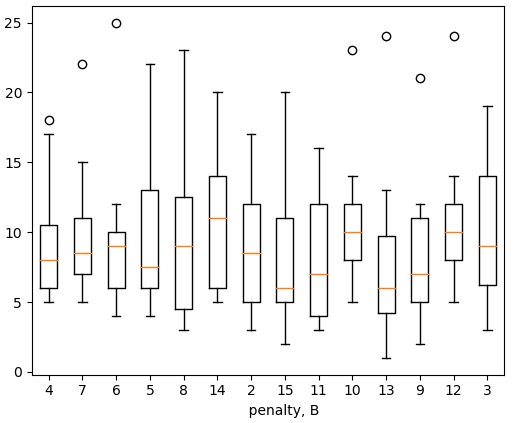
\includegraphics[scale=0.4]{imgs/boxplot_linreg_waiting_pi3.png}
    \caption{Waiting time boxplot for $\Theta=3$ and $B$ values in the range 2 to 15}
    \label{fig:boxplot_linreg}
\end{figure}

The OP policy requires two parameter values, one for the error sum threshold and one for the penalty value. The boxplot analysis was performed by specifying a threshold $\Theta$ for the OP policy and running the simulation with penalty values ranging from 2 to 15. 

In Figure \ref{fig:boxplot_linreg} for the USV sensor "pi3" is shown that the highest mean on update delay is achieved using a threshold $\Theta = 3$ and a penalty value $B=14$.
These values are then used in the complete simulation of the policy comparison. The absolute error rate and the communication rate for each policy are depicted in Figure \ref{fig:err_lin_reg_pi3} and Figure \ref{fig:comm_lin_reg_pi3} respectively.

% place plot of all policies abs error rate for lin reg
\begin{figure}[h]
    \centering
    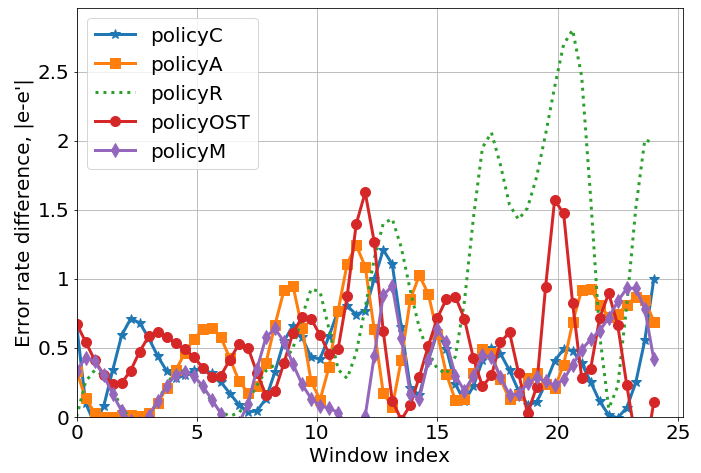
\includegraphics[scale=0.33]{imgs/lin_reg_pi3_w25.png}
    \caption{Absolute error difference for USV sensor system, s=pi3, w=25, using Linear Regression}
    \label{fig:err_lin_reg_pi3}
\end{figure}

\begin{figure}[h]
    \centering
    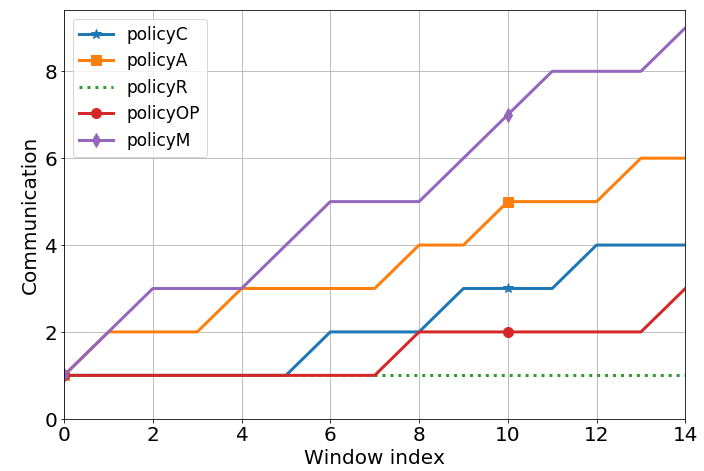
\includegraphics[scale=0.33]{imgs/comm_lin_reg_pi3.png}
    \caption{Communication for USV sensor system, s=pi3, w=25, using Linear Regression}
    \label{fig:comm_lin_reg_pi3}
\end{figure}

As can be seen from Figure \ref{fig:err_lin_reg_pi3}, the plot is very inconsistent due to the low accuracy of the linear regression models. The absolute error difference for the optimal policy preserves a similar rate to policy A for 6 iterations which is aimed at keeping the most accurate model. However, as seen in Figure \ref{fig:comm_lin_reg_pi3}, the optimal policy waits 6 iterations more compared to policy A before sending an update.  

The number of iterations between two model updates are referred to as waiting times and they are further investigated by performing an ANOVA test and a Tukey's HSD test for multiple mean differences. 

\begin{table}[h]
\centering
\begin{tabular}{|l|l|l|}
\hline
\multicolumn{3}{|c|}{\cellcolor[HTML]{DAE8FC}\textbf{ANOVA test results}}       \\ \hline
\multicolumn{3}{|l|}{\cellcolor[HTML]{FFFFFF}\textbf{p-value for waiting time}} \\ \hline
% pi3    & 1.2483606116074772e-30   & \textless{}= 0.05                           \\ \hline
% pi4    & 7.892553014202059e-14    & \textless{}= 0.05                           \\ \hline
pi3           & 1.248e-30         & \textless{}= 0.05                           \\ \hline
pi4           & 7.893e-14         & \textless{}= 0.05                           \\ \hline
\multicolumn{3}{|l|}{\cellcolor[HTML]{FFFFFF}\textbf{p-value for abs error}}    \\ \hline
% pi3    & 1.2436387993444255e-13   & \textless{}= 0.05                           \\ \hline
% pi4    & 2.7228117694830134e-17   & \cellcolor[HTML]{FFFFFF}\textless{}= 0.05   \\ \hline
pi3           & 1.244e-13         & \textless{}= 0.05                           \\ \hline
pi4           & 2.723e-17         & \cellcolor[HTML]{FFFFFF}\textless{}= 0.05   \\ \hline
\end{tabular}
\end{table}

The results show p-values less than 5\% which point to a statistically significant difference between the policy means for sensors "pi3" and "pi4" on their waiting times and absolute error rates. We perform a follow-up Tukey HSD test, which compares the means for each couple of policies and the results are plotted in Figure \ref{fig:lin_reg_pi3_waiting_plot_diff_means} and Figure \ref{fig:lin_reg_pi3_error_plot_diff_means}.

The plot in Figure \ref{fig:lin_reg_pi3_waiting_plot_diff_means} shows that optimal policy has a statistically significant higher waiting time compared to policy M, policy C and policy A and the same mean with the Random policy as intended.
This shows the advantage in communication reduction introduced by the optimal policy.
Moreover, we perform the Tukey's HSD test on the absolute error difference of each policy obtained during the simulation along with policy E. Policy E communicates the up-to-date models on each iteration and is intended as a lower bound which show the absolute error rate of the models at its lowest. 

The results in Figure \ref{fig:lin_reg_pi3_error_plot_diff_means} show that the accuracy of the models does not suffer a significant deterioration compared to policy E and the other communication reduction policies but preserves the highest postponing time. Moreover, the plot shows that randomly updating the models leads to a significant increase in the absolute error, therefore, the optimal policy does not just correctly guess the optimal number of updates but also the optimal time between the updates. 
% talk about one-way anova results and tukey ttest on waiting time
% place plot
\begin{figure}[h]
    \centering
    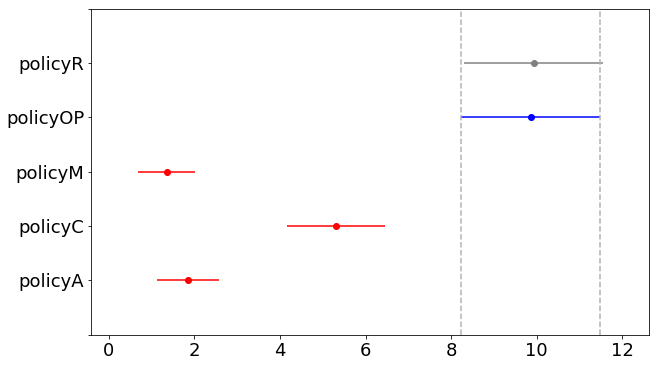
\includegraphics[scale=0.35]{imgs/lin_reg_pi3_waiting_plot_diff_means.png}
    \caption{Policy comparison on waiting time using using Linear Regression}
    \label{fig:lin_reg_pi3_waiting_plot_diff_means}
\end{figure}
% talk about one way anova results and tukey ttest on abs error rate
\begin{figure}[h]
    \centering
    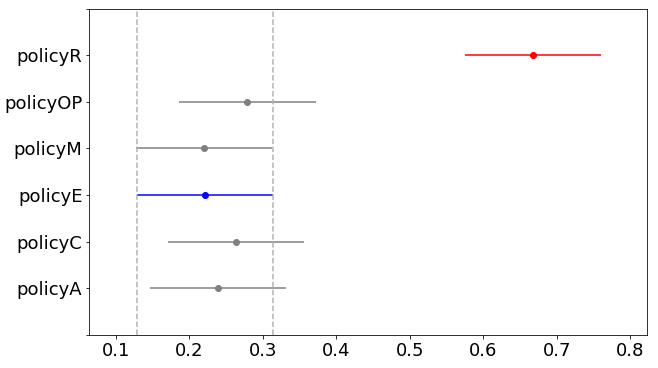
\includegraphics[scale=0.35]{imgs/lin_reg_pi3_error_plot_diff_means.png}
    \caption{Policy comparison on absolute error rate time using Linear Regression}
    \label{fig:lin_reg_pi3_error_plot_diff_means}
\end{figure}

\subsection{Experimentation with Support Vector Regression models}

After some analysis of the data it was found that the initial 100 datapoints of the HT sensor dataset contain a single drift in the observed pattern. However, the rest of the data used in the simulation of the online algorithm has no noticeable changes, which results in no communication between the edge node and the gateway. This called for placing an artificial change in the data. One incremental long term change and one abrupt short term change affecting only the MOX sensor data and preserving the genuine datastream for the humidity and temperature. This is aimed to simulate a new pattern in the data which will cause a change in the communicated models.

The incremental long term change occurs from iteration 50 of the start of the simulation, where the MOX sensor values are increased with 10\% of the mean value in the next 12 iterations and after that the change is kept persistent throughout the rest of the simulation. This drift in the data is intended to serve as a critical change \cite{lautay2018} which should be detected by the algorithm and acted upon as soon as possible.

The second abrupt short term change occurs in iteration 108. The change in the MOX sensor values is increased with 2.5\% of the mean value and then decreased to the genuine datastream in the next 4 iterations. This drift in the data is intended to serve as a nuisance change \cite{lautay2018} which should be of least importance to the algorithm.

The global parameters for this experiment are set the same way as in the experimentation using the linear regression models: window size 25 and initial preprocessing data containing 100 datapoints. 
The Median policy uses the $\alpha$ with a set value of 0.5 and the cumulative sum threshold for the CuSum policy is set to $\Theta=0.5$.

\begin{figure}[h]
    \centering
    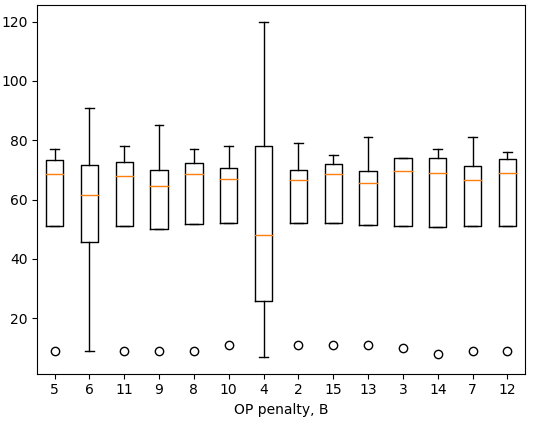
\includegraphics[scale=0.4]{imgs/boxplot_svr_waiting_R5.png}
    \caption{Waiting time boxplot for $\Theta=1$ and $B$ values in the range 2 to 15}
    \label{fig:boxplot_svr}
\end{figure}

For the optimal policy, the cumulative sum threshold was set to $\Theta=1$ as it allowed the needed sensitivity for the detection of the critical change. The boxplot in Figure \ref{fig:boxplot_svr} shows the waiting times when performing the simulation for MOX sensor R5 using penalty values in the range 2 to 15. The highest mean waiting time is achieved using penalty $B=3$. The simulation results using this setting is depicted in Figure \ref{fig:err_rbf_svr_R5} and Figure \ref{fig:comm_rbf_svr_R5}.

\begin{figure}[h]
    \centering
    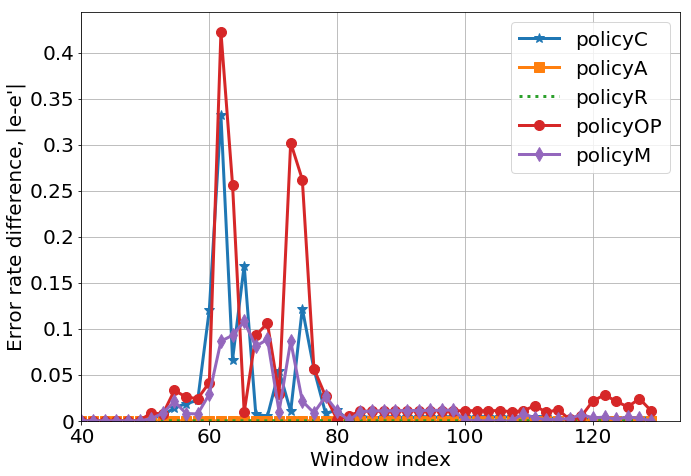
\includegraphics[scale=0.33]{imgs/svr_rbf_R5_w25.png}
    \caption{Absolute error difference for HT sensor system, s=R5, w=25,
    using Support Vector Regression with RBF Kernel 
    given an artificial change at 40th window iteration}
    \label{fig:err_rbf_svr_R5}
\end{figure}

In Figure \ref{fig:err_rbf_svr_R5}, the absolute error line is distorted as expected after the critical change and less affected after the nuisance change. The error appears to increase the most for the CuSum policy and the optimal policy and less for the Median policy. An interesting observation is that the policy relying only on the accuracy appears to be persistently close to 0, which can be explained by the good quality predictions the SVR model delivers.

\begin{figure}[h]
    \centering
    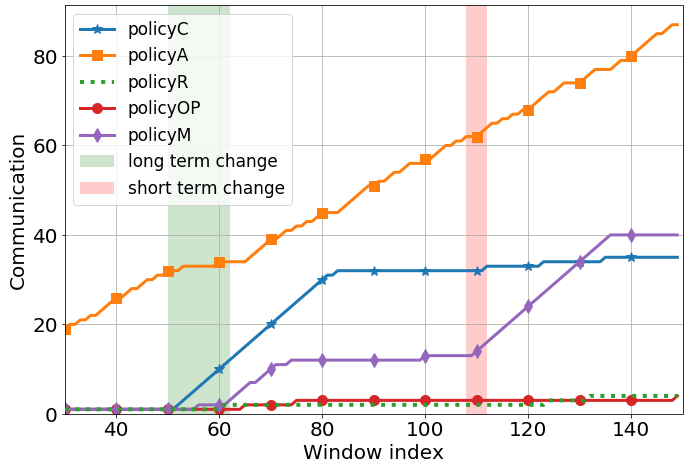
\includegraphics[scale=0.34]{imgs/comm_svr_rbf_R5.png}
    \caption{Communication for HT sensor system, s=R5, w=25, using Support Vector Regression with RBF Kernel}
    \label{fig:comm_rbf_svr_R5}
\end{figure}

However, when we focus our attention to the communication rate of the policies in Figure \ref{fig:comm_lin_reg_pi3}. Despite the allowed error by the CuSum policy, the critical change appears to cause a communication overhead mid and post change, where even the Median policy manages to decrease the absolute error at the cost of less communication. On the contrary, the optimal policy allows a high error rate but at the cost of just two sent messages as a result of the critical change, which happens shortly after the change and the nuisance change causes an updated model about 40 iterations after the change.

The waiting times for each policy is investigated further again by performing an ANOVA test and a Tukey's HSD test for multiple mean differences.

\begin{table}[h]
\centering
\begin{tabular}{|l|l|l|}
\hline
\multicolumn{3}{|c|}{\cellcolor[HTML]{DAE8FC}\textbf{ANOVA test results}}       \\ \hline
\multicolumn{3}{|l|}{\cellcolor[HTML]{FFFFFF}\textbf{p-value for waiting time}} \\ \hline
% R3    & 9.198283524237108e-18     & \textless{}= 0.05                           \\ \hline
% R5    & 1.4772473722529788e-32    & \textless{}= 0.05                           \\ \hline
R3                 & 9.198e-18     & \textless{}= 0.05                           \\ \hline
R5                 & 1.477e-32    & \textless{}= 0.05                           \\ \hline
\multicolumn{3}{|l|}{\cellcolor[HTML]{FFFFFF}\textbf{p-value for abs error}}    \\ \hline
% R3    & 6.003242592652264e-23     & \textless{}= 0.05                           \\ \hline
% R5    & 1.0617164482428442e-11    & \cellcolor[HTML]{FFFFFF}\textless{}= 0.05   \\ \hline
R3                 & 6.003e-23     & \textless{}= 0.05                           \\ \hline
R5                 & 1.062e-11    & \cellcolor[HTML]{FFFFFF}\textless{}= 0.05   \\ \hline
\end{tabular}
\end{table}

The ANOVA test produces p-values less than 5\% which show that there is a statistically significant difference between the means of the waiting time and the absolute error for sensors "R3" and "R5". Since the hypothesis that the policy means were the same was rejected, we performed the Tukey's HSD test with results plotted in Figure \ref{fig:svr_rbf_R5_waiting_plot_diff_means} and Figure \ref{fig:svr_rbf_R5_error_plot_diff_means}.

\begin{figure}[h]
    \centering
    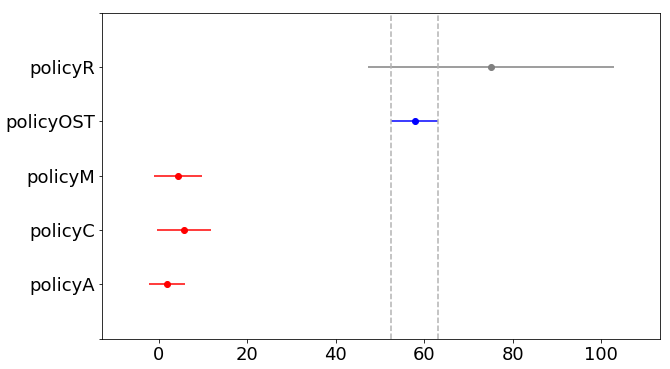
\includegraphics[scale=0.35]{imgs/svr_rbf_R5_waiting_plot_diff_means.png}
    \caption{Policy comparison on waiting time using Support Vector Regression with RBF Kernel}
    \label{fig:svr_rbf_R5_waiting_plot_diff_means}
\end{figure}

% talk about one way anova results and tukey ttest on abs error rate
\begin{figure}[h]
    \centering
    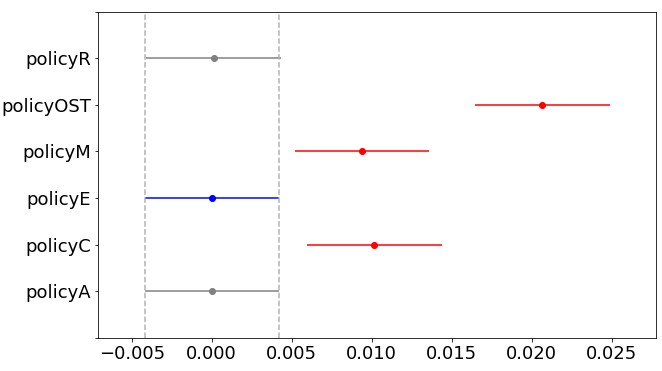
\includegraphics[scale=0.35]{imgs/svr_rbf_R5_error_plot_diff_means.png}
    \caption{Policy comparison on absolute error rate time using Support Vector Regression with RBF Kernel}
    \label{fig:svr_rbf_R5_error_plot_diff_means}
\end{figure}

The plots show a significantly higher waiting time for the optimal policy but also a very high error rate compared to the base accuracy of policy E in Figure \ref{fig:svr_rbf_R5_error_plot_diff_means}. Analysing the results shows that the basic Median policy performs better than both the CuSum and the optimal policy with regards to communication and error rate.
\newpage
\subsection{Evaluation Summary}
% place table with all policies and say when each is good for accurate models and when is good to wait and so on
The results of this experiment can be concluded in a summarised table which shows the trade-offs for each policy and the situations in which each one is recommended. 
For example, when dealing with models which have high quality predictions over data of a small window, if we are willing to sacrifice some of the accuracy then a basic policy such as the Median policy can deliver the wanted results. However, if the models are to be used occasionally without pressing short term deadlines then the Optimal Postponing algorithm will eventually deliver the up-to-date accurate models and will prevent a communication overhead.

On the contrary, if the generated models are expected to produce low quality predictions, then the cusum policy and especially the optimal policy are viable options. They will reduce the communication between the sensing nodes and the edge gateway but will preserve the initial quality of the contextual data.

\begin{table}[h]
\begin{tabular}{|l|l|l|}
\hline
\rowcolor[HTML]{c1fbc0} 
\multicolumn{1}{|c|}{\cellcolor[HTML]{c1fbc0}Policy} & \multicolumn{1}{c|}{\cellcolor[HTML]{c1fbc0}\begin{tabular}[c]{@{}c@{}}High quality \\ predictions\end{tabular}} & \multicolumn{1}{c|}{\cellcolor[HTML]{c1fbc0}\begin{tabular}[c]{@{}c@{}}Low quality \\ predictions\end{tabular}} \\ \hline
\textbf{policy C}& \begin{tabular}[c]{@{}l@{}}high error and \\ high communication\end{tabular}& \checkmark\\ \hline
\textbf{policy M}& \checkmark& \begin{tabular}[c]{@{}l@{}}high \\ communication\end{tabular}\\ \hline
\textbf{policy OP}& high error& \checkmark\\ \hline
\textbf{policy A}& \checkmark& \begin{tabular}[c]{@{}l@{}}high \\ communication\end{tabular}\\ \hline
\end{tabular}
\end{table}

\section{Conclusions}
This paper presented and evaluated a decision technique for optimal model update postponing at the edge. The results showed that the algorithm preserves the accuracy of the generated models and significantly reduces the communication overhead for linear regression models. However, when applying the technique with models of higher prediction quality, the quality of the models deteriorates due to the low communication rate. In this case, the technique should be used only in scenarios which do not require constant access to the most up-to-date contextual data. 


{\bf Acknowledgments.}
I would like to thank my supervisor Dr Christos Anagnostopoulos for the guidance and support in the past two years. I would not have managed to achieve so much without the enthusiasm, motivation and endless opportunities he provided me with. I would also like to thank my parents who comforted me throughout all the hardship living far from home has brought me and my friends who helped me feel at home no matter where I was.

\bibliographystyle{abbrv}
\bibliography{example.bib}

\begin{appendix}
% \section{CUSUM policy}\label{baddist}
% \begin{algorithm}[h]
% \caption{Function to Obtain Bad Distribution}
% \begin{algorithmic}
% \Function{obtainBadDist}{}
%     \State $X, y \gets$ fromDataStream
%     \State $model \gets$ fit($X,y$)
%     \For{$i = 0$ \textbf{to} $100$}
%         \State $X, y \gets$ fromDataStream
%         \State $newModel \gets$ fit($X,y$)
%         \State $mse \gets$ calcError($model,X,y$)
%         \State $msePrime \gets$ calcError($newModel,X,y$)
%         \State $absMse \gets \mid error - msePrime \mid$
%         \State $absoluteMseVector$.append($absMse$)
%     \EndFor
%     \State $mean \gets$ calcMean($absoluteMseVector$)
%     \State $variance \gets$ calcVar($absoluteMseVector$)
%     \State $shapeBad \gets mean^2/variance$
%     \State $scaleBad \gets variance/mean$
%     \State $badDist \gets$ Gamma($shapeBad, scaleBad$)\\
%     \Return $badDist$
% \EndFunction
% \end{algorithmic}
% \end{algorithm}
\section{CUSUM policy}\label{baddist}
\begin{algorithm}[H]
\caption{Function to Obtain Bad Distribution}
\begin{algorithmic}
\Function{obtainBadDist}{}
    \State \textbf{receive}($X, y$)
    \State $model \gets$ \textbf{fit}($X,y$)
    \State $\textbf{z} \gets \emptyset$
    \For{$t \gets 1$ \textbf{to} $T$}
        \State \textbf{receive}($X, y$)
        \State $newModel \gets$ \textbf{fit}($X,y$)
        \State $e \gets$ \textbf{error}($model,X,y$)
        \State $e' \gets$ \textbf{error}($newModel,X,y$)
        \State $Z \gets \mid e - e' \mid$
        \State $\textbf{z} \gets \textbf{z} \cup \{Z\}$
    \EndFor
    \State $\mu \gets$ \textbf{mean}($\textbf{z}$)
    \State $\sigma^2 \gets$ \textbf{var}($\textbf{z}$)
    \State $shape \gets \mu^2/\sigma^2$
    \State $scale \gets \sigma^2/\mu$\\
    \Return Gamma($shape, scale$)
\EndFunction
\end{algorithmic}
\end{algorithm}

% \section{CUSUM policy}\label{gooddist}
% \begin{algorithm}[h]
% \caption{Function to Obtain Good Distribution}
% \begin{algorithmic}
% \Function{obtainGoodDist}{}
%     \State $X, y \gets$ fromDataStream
%     \State $model \gets$ fit($X,y$)
%     \For{$i = 0$ \textbf{to} $100$}
%         \State $X, y \gets$ fromDataStream
%         \State $newModel \gets$ fit($X,y$)
%         \State $mse \gets$ calcError($model,X,y$)
%         \State $msePrime \gets$ calcError($newModel,X,y$)
%         \State $absMse \gets \mid error - msePrime \mid$
%         \State $absoluteMseVector$.append($absMse$)
%         \State $model \gets newModel$
%     \EndFor
%     \State $mean \gets$ calcMean($absoluteMseVector$)
%     \State $variance \gets$ calcVar($absoluteMseVector$)
%     \State $shapeGood \gets mean^2/variance$
%     \State $scaleGood \gets variance/mean$
%     \State $goodDist \gets$ Gamma($shapeGood, scaleGood$)\\
%     \Return $goodDist$
% \EndFunction
% \end{algorithmic}
% \end{algorithm}

\section{CUSUM policy}\label{gooddist}
\begin{algorithm}[H]
\caption{Function to Obtain Good Distribution}
\begin{algorithmic}
\Function{obtainGoodDist}{}
    \State \textbf{receive}($X, y$)
    \State $model \gets$ \textbf{fit}($X,y$)
    \State $\textbf{z} \gets \emptyset$
    \For{$t \gets 1$ \textbf{to} $T$}
        \State \textbf{receive}($X, y$)
        \State $newModel \gets$ \textbf{fit}($X,y$)
        \State $e \gets$ \textbf{error}($model,X,y$)
        \State $e' \gets$ \textbf{error}($newModel,X,y$)
        \State $Z \gets \mid e - e' \mid$
        \State $\textbf{z} \gets \textbf{z} \cup \{Z\}$
        \State $model \gets newModel$
    \EndFor
    \State $\mu \gets$ \textbf{mean}($\textbf{z}$)
    \State $\sigma^2 \gets$ \textbf{var}($\textbf{z}$)
    \State $shape \gets \mu^2/\sigma^2$
    \State $scale \gets \sigma^2/\mu$\\
    \Return Gamma($shape, scale$)
\EndFunction
\end{algorithmic}
\end{algorithm}

% \section{Time-optimised Policy}\label{rewarddist}
% \begin{algorithm}[h]
% \caption{Obtain Reward Distribution}
% \begin{algorithmic}
% \Function{obtainRewardDist}{}
%     \State $X, y \gets$ fromDataStream
%     \State $model \gets$ fit($X,y$)
%     \State $absoluteSum \gets 0$
%     \For{$i = 0$ \textbf{to} $100$}
%         \State $X, y \gets$ fromDataStream
%         \State $newModel \gets$ fit($X,y$)
%         \State $mse \gets$ calcError($model,X,y$)
%         \State $msePrime \gets$ calcError($newModel,X,y$)
%         \State $absMse \gets \mid error - msePrime \mid$
%         \State $absoluteSum \gets absoluteSum + absMse$
%         \State $absoluteMseVector$.append($absMse$)
        
%         \If{$absoluteSum \leq \Theta$}
%             \State $V_t \gets t$
%         \Else
%             \State $V_t \gets -B$
%         \EndIf
%     \EndFor
%     \State $mean \gets$ calcMean($absoluteMseVector$)
%     \State $variance \gets$ calcVar($absoluteMseVector$)
    
%     \State $shapeReward \gets mean^2/variance$
%     \State $scaleReward \gets variance/mean$\\
%     \Return Gamma($shapeReward, scaleReward$)
    
% \EndFunction
% \end{algorithmic}
% \end{algorithm}
\newpage
\section{Time-optimised Policy}\label{rewarddist}
\begin{algorithm}[H]
\caption{Obtain Reward Distribution}
\begin{algorithmic}
\Function{obtainRewardDist}{}
    \State \textbf{receive}($X, y$)
    \State $model \gets$ \textbf{fit}($X,y$)
    \State $S \gets 0$
    \State $\textbf{z} \gets \emptyset$
    \For{$t \gets 1$ \textbf{to} $T$}
        \State \textbf{receive}($X, y$)
        \State $newModel \gets$ \textbf{fit}($X,y$)
        \State $e \gets$ \textbf{error}($model,X,y$)
        \State $e' \gets$ \textbf{error}($newModel,X,y$)
        \State $Z \gets \mid e - e' \mid$
        \State $S \gets S + Z$
        \State $\textbf{z} \gets \textbf{z} \cup \{Z\}$
        \If{$S > \Theta$}
            \State $S \gets Z$
        \EndIf
    \EndFor
    \State $\mu \gets$ \textbf{mean}($\textbf{z}$)
    \State $\sigma^2 \gets$ \textbf{var}($\textbf{z}$)
    \State $shape \gets \mu^2/\sigma^2$
    \State $scale \gets \sigma^2/\mu$\\
    \Return Gamma($shape, scale$)
    
\EndFunction
\end{algorithmic}
\end{algorithm}

\end{appendix}


\end{document}